\documentclass[eng, 11pt, twoside, openany]{mgr}
% draft

\usepackage{hyperref}
\usepackage{polski}
\usepackage[utf8]{inputenc}
\usepackage{graphicx}
% \usepackage{latexsym}
% \usepackage{afterpage}

\author{Marcin Bober}
\title{Projekt systemu sensorycznego bazującego na protokole MQTT}
\engtitle{Design a sensor system based on MQTT protocol}
\supervisor{Dr inż., Mateusz Cholewiński, K29W04D02}
\field{Automatyka i Robotyka (AIR)}
\specialisation{Robotyka (ARR)}
\date{2021}


\begin{document}
  \bibliographystyle{plabbrv}
  \maketitle
  \tableofcontents
  
  \chapter{Wprowadzenie}
  
    Celem pracy jest stworzenie systemu sensorycznego 
    potrafiącego zarządzać silnikiem prądu stałego.

    % dopisać 1-2 lania wody 
  

    \section{Założenia}

      System składa się z urządzenia wykonawczego serwera 
      oraz aplikacji dostępowej. 
      Komunikacja pomiędzy elementami systemu 
      następuje poprzez serwer z wykorzystaniem protokołu MQTT.
      
      Urządzenie wykonawcze składa się z mikrokontrolera,
      mostka H oraz silnika prądu stałego wyposarzonego w enkoder
      kwadraturowy. Oprócz tego posiada układ pomiaru napięcia, a
      także wszystkie elementy niezbędne do prawidłowej pracy 
      procesora.

      Aplikacja dostępowa służy do łaczenia się z serwerem 
      poprzez protokół MQTT. Ma za zadanie stanowić prosty i 
      przejrzysty interfejs do sterowania urządzeniem.
      Za jej pomocą mamy możliwość:
  
      \begin{itemize}
        \item zadawania prędkości obrotowej silnika,
        \item odczytu aktualnej prędkości silnika,
        \item zmiany nastaw regulatora PID,
        \item odczytu napięcia zasilania urządzenia,
        \item odczytu wypełnienia sygnału PWM.
      \end{itemize}
  
      Ostatnim elementem systemu jest serwer hostujący broker
      komunikatów w protokole MQTT. Ma on za zadanie być
      pośrednikiem w komunikacji między aplikacją dostępową,
      a urządzeniem wykonawczym.

    \section{Opis komponentów}

      \subsection{Aplikacja dostępowa}
        W celu komfortowej obsługi sterownika silnika,
        zdecydowałem się na stworzenie aplikacji dostępowej w 
        języku C++, która będzie komunikowała się w protokole MQTT.
        W tym celu wykorzystałem otwarto źródłową wersję narzędzia
        programistyczne jakim jest QT \cite{qt}. 
        Moja decyzja była uwarunkowana moją szeroką znajomością
        tego narzędzia. Ponadto biblioteki QT posiadają dobrze 
        zefiniowane warstwy abstrakcji oraz bardzo wylewną 
        dokumentację, co sprawia że tworzenie zawansowanych, 
        przenośnych aplikacji okienkowych jest wybitnie proste i 
        przyjemne. 

      \subsection{Urządzenie wykonawcze}
        Urządzenie końcowe zostało oparte na ogromnie popularnym
        SoC ESP32-S, chińskiej firmy Espressif Systems. 
        Został on wybrany ze względu na wbudowany moduł WiFi oraz
        bardzo niską cene wynoszącą poniżej 2\$ za sztukę. 
        Ponadto oferuje on:

        \begin{itemize}
          \item dwurdzeniowy procesor o taktowaniu do 240MHz,
          \item 320 KiB RAM, 448 KiB ROM,
          \item Bluetooth w standardzie 4.2 oraz BLE,
          \item 34 wyprowadzenia GPIO.
        \end{itemize}


        \begin{figure}[ht]
          \centering
          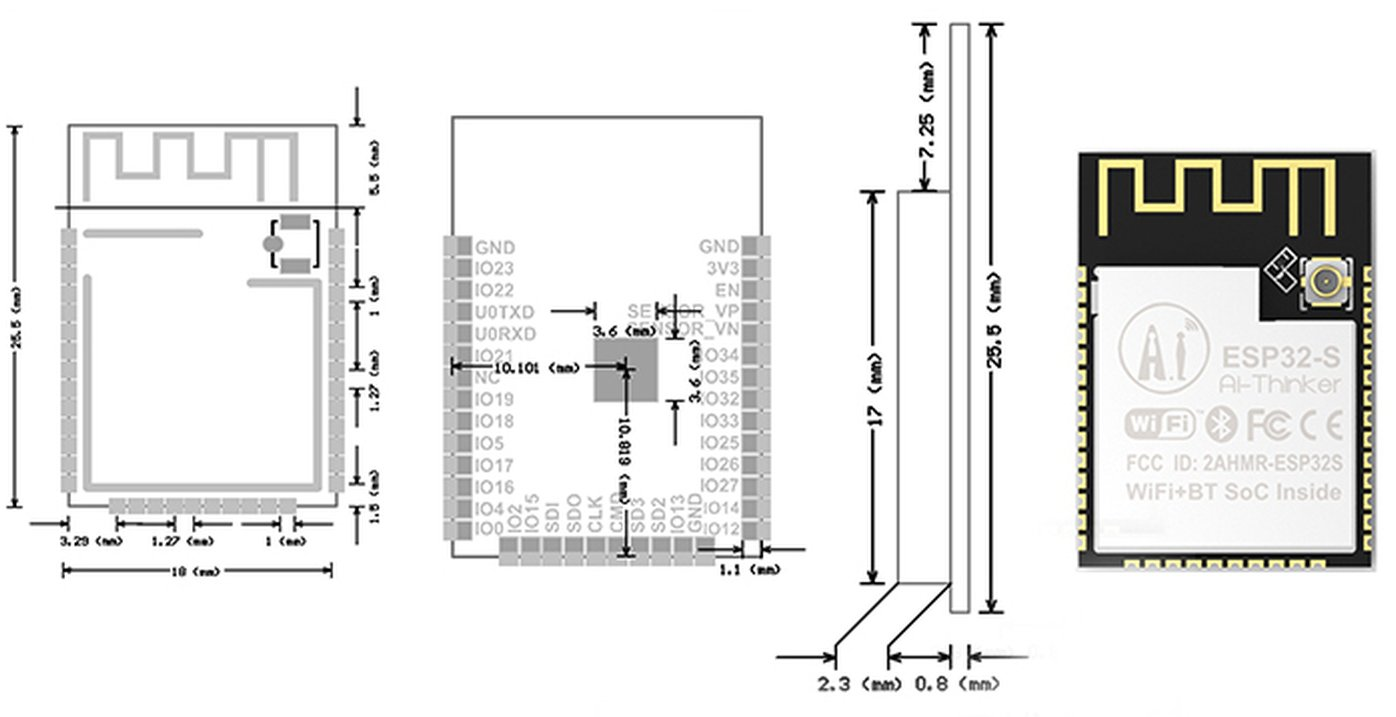
\includegraphics[width=0.5\textwidth]{img/esp32.jpg}
          \caption{Schemat wykorzystanej jednostki centralnej}
        \end{figure}

        Można zauważyć że posiada on dość imponujące parametry 
        jak na tak tani produkt. Pozwoli to na zadowalającą wydajność
        całego systemu bez obaw o niewystarczające zasoby lub 
        kiepską optymalizację.

        W roli mostka H zastosowałem bardzo popularny układ scalony
        L298N w obudowie Multiwatt15. Nie jest to najdoskonalszy wybór,
        ale zdecydowanie wystarczający dla tego zastosowania. 
        Może się on poszczycić napięciem zasilania silników do 46V i 
        prądem szczytowym na poziomie 2A. Ma on dwa kanały co sprawia że
        może jednocześnie sterować dwoma osobnymi silnikami, jednakże
        mój projekt zakłada wykorzystanie tylko jednego silnika, więc 
        drugi kanał pozostanie nieaktywny. Układ tego typu znacząco
        redukuje poziom skomplikowania urządzenia ponieważ, aby
        go uruchomić wystarczą cztery diody i kondensator filtrujący 
        napięcie. \cite{mostek}


        \begin{figure}[ht]
          \centering
          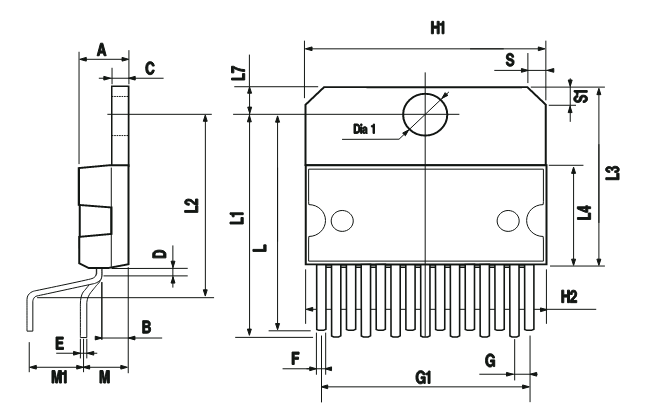
\includegraphics[width=0.5\textwidth]{img/h_bridge.png}
          \caption{Schemat wykorzystanego mostka H}
        \end{figure}


        Silnik jest to bardzo konkurencyjnie wyceniany produkt 
        firmy DFROBOT. Został on wybrany w głównej mierze
        ze względu na swoją niską cene i parametry które w zupełności
        wystarczą do zeralizowania tego projektu.
        Jest on wyposażony w metalową przekładnię zapewniającą
        przełożenie napędu w proporcji 20:1. Ponadto, na końcu
        silnika jest fabrycznie zamontowany enkoder kwadraturowy,
        który produkuje 11 impulsów na każdy obrót wału głównego.
  

        \begin{figure}[ht]
          \centering
          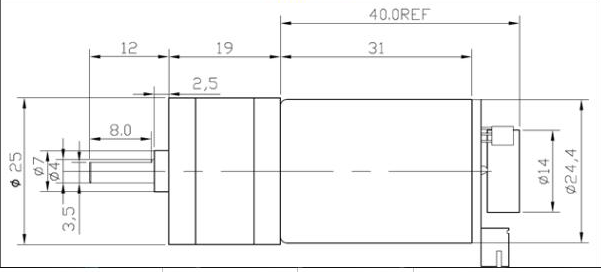
\includegraphics[width=0.5\textwidth]{img/silnik.png}
          \caption{Schemat wykorzystanego silnika}
        \end{figure}




      \subsection{Serwer}
        Ostatnim elementem projektu jest Broker MQTT. Jego zadaniem jest
        bycie łącznikiem pomiędzy urządzeniami. Pozwala on na łatwe
        subskrybowanie jak i publikowanie informacji. Ja zdecydowałem się 
        na użycie w tej roli otwartoźródłowego brokera Mosquitto od fundacji 
        Eclipse. Jest to jeden z popularniejszych programów tego typu, a
        zawdzięcza to małym wymaganiom sprzętowym, skalowalności oraz
        dostępności na wielu architekturach. 
        
        % Co więcej, w celu wdrożenia
        % przenośności projektu, postanowiłem poddać broker MQTT konteneryzacji,
        % dzięki czemu można łatwo prznosić go na inne komputery wraz z całą 
        % konfiguracją przy użyciu programu Docker.

  \chapter{Schemat działania projektu}
        diagram wymiany danych, tematów mqtt 

  \chapter{Szczegółowy opis sterownika}
    \section{System operacyjny}
      jaki? po co? 

    \section{System operacyjny}
      użyty framework

        
    \section{Schemat funkcionowania}
      diagram wątków, kolejki

    \section{Regulator PID}
      implementacja, dobór nastaw

    \section{Pomiar napięcia}
      implementacja, regresja liniowa, błędy pomiarowe

    \section{Łączenie z brokerem}
      implementacja, 

  \chapter{Szczegółowy opis brokera MQTT}
    \section{Sposób działania}
      sposób działania,

    \section{Implementacja i konfiguracja}
      docker, konfiguracja

  \chapter{Szczegółowy opis aplikacji dostępowej}
    \section{Wykorzystana technologia}
        Qt

    \section{Implementacja komunikacji}
      \subsection{Odbiór danych}
      \subsection{Wysyłanie danych}
    \section{Wykresy}


  \chapter{Instrukcja obsługi}

  \chapter{Podsumowane}

  \addcontentsline{toc}{chapter}{\bibname}
  
  
  \begin{thebibliography}{9}

    \bibitem{qt}
      Qt Development Frameworks: Dokumentacja biblioteki Qt \newline
      \url{https://doc.qt.io/qt-5/} \newline
      Dostęp 14.09.2021

    \bibitem{mostek}
      STMicroelectronics: Dokumentacja L298H \newline
      \url{https://www.sparkfun.com/datasheets/Robotics/L298_H_Bridge.pdf} \newline
      Dostęp 14.09.2021

    \bibitem{esp32}
      Espressif Systems: Dokumentacja ESP32
      \url{https://www.espressif.com/sites/default/files/documentation/esp32_datasheet_en.pdf} \newline
      Dostęp 14.09.2021
      
    \bibitem{mqtt}
      OASIS: Dokumentacja standardu MQTT 5.0 \newline
      \url{https://docs.oasis-open.org/mqtt/mqtt/v5.0/mqtt-v5.0.pdf} \newline
      Dostęp 14.09.2021
    
    \bibitem{mostek}
      V.P. Eloranta, J. Koskinen, M. Leppanen, V. Reijonen: 
      Designing Distributed Control Systems: A Pattern Language Approach, 
      Wiley, 2014.
      
  \end{thebibliography}


  \listoffigures

\end{document}